\documentclass[12pt]{article}
\usepackage{sbc-template}
%  \usepackage{subfigure}
%\usepackage{graphicx,url}
\usepackage[utf8]{inputenc}
\usepackage[brazil]{babel}
\usepackage{rotating}
%  \usepackage{subfigure}
\usepackage{chngcntr}
% \usepackage{subcaption}
\usepackage[a4paper]{geometry}
\geometry{top=3 cm,bottom=3cm,left=2.5cm,right=3cm}

% \usepackage[font=small]{caption}
%\usepackage[brazil]{babel}   
%\usepackage[latin1]{inputenc}  
%\usepackage{color}
%\usepackage[usenames,dvipsnames, table]{xcolor}
\usepackage{listings}
% \usepackage{caption}   
% \captionsetup[figure]{labelsep=endash,labelfont=bf,textfont=bf}
% \captionsetup[table]{labelsep=endash,labelfont=bf,textfont=bf}
%\usepackage[most]{tcolorbox}

% Números das páginas em algarismos romanos
\pagenumbering{arabic}
\usepackage{lipsum}
\newcommand{\aspas}[1]{{``#1''}}
\newcommand{\aspassimples}[1]{{`#1'}}
\usepackage{enumerate}
\usepackage{hyperref}
\usepackage{booktabs}
\usepackage{soul}
\usepackage{setspace}
\usepackage{graphicx}
\usepackage{scrextend}
\usepackage{makeidx}
\usepackage{tabularx} % nice to have
\usepackage{array}


% % Muda as margens
% \addtolength{\oddsidemargin}{-.875in}
% 	\addtolength{\evensidemargin}{-.875in}
% 	\addtolength{\textwidth}{1.75in}

% 	\addtolength{\topmargin}{-.875in}
% 	\addtolength{\textheight}{1.75in}

\usepackage{float}
\usepackage{bm}
\usepackage{booktabs} % necessary for style
\usepackage{setspace}
\usepackage{fancy-listings}
\usepackage{colortbl}
\usepackage[table]{xcolor}  
\usepackage{adjustbox}
\usepackage{tabularx}
\usepackage{graphicx}
\usepackage{multirow}
%\newcommand{\mcode}[1]{$\mathtt{#1}$}
\newcommand*{\mcode}[1]{%
$\mathtt{#1}$%
}
%\newcommand{\mcode}[1]{\texttt{#1}}

\urlstyle{rm}
\sloppy

%\title{Um Processo de Conformidade Arquitetural voltado à Arquitetura de Microsserviços}
\title{\textcolor{blue}{Conciliation Bank Application}:\\{\large \textcolor{blue}{Check the communication and structural design conformance}}}
%(Empresa Equals)}
%\title{ Resultado da aplicação da ferramenta DCL$^+$ na Empresa Equals}

% \author{Elena A. Araujo, Álvaro Espíndola and Ricardo}
% %{Elena A. Araujo, Ricardo Terra}

% \address{Universidade Federal de Lavras, Lavras, Brasil 
% \email{elena.araujo@posgrad.ufla.br}
% }


\definecolor{bostonuniversityred}{rgb}{0.8, 0.0, 0.0}
\definecolor{blue(pigment)}{rgb}{0.2, 0.2, 0.6}
\definecolor{verdeescuro}{rgb}{0.0, 0.44, 0.0}
\renewcommand{\lstlistingname}{Listagem}
\lstdefinestyle{colorido}{
        numbers=left,
        numberstyle=\tiny, 
        stepnumber=1,
        numberfirstline=auto,
        firstnumber=auto,
        captionpos=b,
        xleftmargin=0.4cm,
        xrightmargin=0.0cm,
        framexbottommargin=0cm,
        framextopmargin=0cm,
        boxpos=c,
        frame=single,
	basicstyle=\linespread{0.85}\ttfamily \scriptsize,
        commentstyle=\itshape\color{darkgreen},
        showstringspaces=true,        
        tabsize=4,
        showstringspaces=true,
        moredelim=**[is][\color{bostonuniversityred}\normalfont\bfseries]{@}{@},
	moredelim=**[is][\normalfont\bfseries\color{blue(pigment)}]{|}{|},
    moredelim=**[is][\normalfont\color{verdeescuro}]{&}{&},
	emph={[1]only,can,cannot,depend,create,access,must,implement,useannotation,communicate, must-communicate, cannot-communicate, can-communicate, module,declare,can-communicate-only, can-depend, can-useannotation, can-throw, can-access-only, can-depend-only, cannot-depend, must-useannotation, cannot-access, must-access,must-implement, can-access, must-depend, must-extend},emphstyle={[1]\bfseries}, 
%xleftmargin=0.3cm,
%xrightmargin=0.3cm,
}




\begin{document} 

\maketitle


\vspace{-0.3cm}
\noindent\textbf{\large{\textcolor{blue}{Architectural design of the microservices of a bank conciliation application}}}
\label{sec:Estruturaltodos}

%--------------------------------------------
\noindent\textbf{\textcolor{blue}{Audit microservice}}
\label{sec:ApendiceAudit}

\vspace{-0.04cm}
%-------------------------------------------
\begin{lstlisting}[style=colorido, caption={\textcolor{blue}{Audit microservice's architectural project specification.}},label={list:especArquiteturalAudit}
]
#Internal modules of the Audit microservice
module Controller: br.com.microservices.audit.controller.*
module Domain: br.com.microservices.audit.domain.*
module Main: br.com.microservices.audit.AuditApplication
module Service: br.com.microservices.audit.services.[a-zA-Z]*Impl

#External modules of the audit microservice
module CtlrAnnotations:  org.springframework.web.bind.annotation.RequestMapping,  org.springframework.web.bind.annotation.RestController
module ExceptBC: br.com.inflexion.SpcInternalException
module MainAnnotations: org.springframework.boot.SpringApplication, org.springframework.boot.context.properties.EnableConfigurationProperties, org.springframework.boot.autoconfigure.SpringBootApplication, org.springframework.cloud.client.discovery.EnableDiscoveryClient
module Apache: org.apache.**
module ServiceAnnotation: org.springframework.stereotype.Service
module CBMultitenancy: br.com.basecommons.MultitenancyProperties
module JPA: javax.persistence.**
module Beans: org.springframework.context.**, org.springframework.beans.**
module Jndi: org.springframework.jndi.**

#Structural Design Constraints  SC's
#Only-can		
only Controller, Service can-depend Service																																							"#SC1"
only Controller can-useannotation CtlrAnnotations																																	"#SC2"
only Service can-depend Jndi																																																						"#SC3"
only Service can-throw ExceptBC																																																			"#SC4"

#Can-only
Main can-access-only Controller, MainAnnotations, Logger, Apache, $java											"#SC5"@*@

#Cannot
Domain cannot-depend JPA																																																										"#SC6"
Main cannot-depend CBMultitenancy																																																	"#SC7"

#Must 
Service must-useannotation ServiceAnnotation																																						"#SC8"
\end{lstlisting}
%--------------------------------------------
%--------------------------------------------
\begin{figure}[ht]
\centering
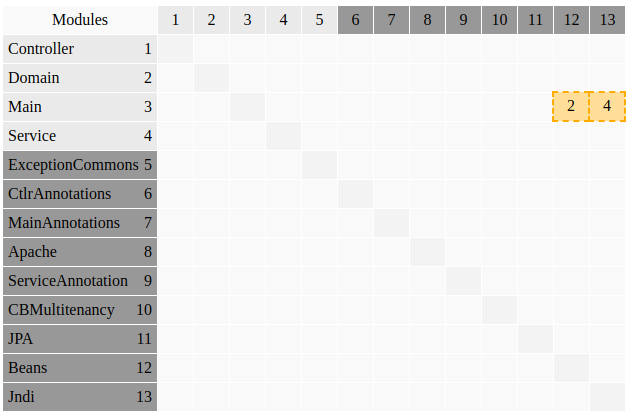
\includegraphics[width=0.6\textwidth]{figuras/violacoesAudit.png}
\caption{\textcolor{blue}{Audit microservice's architectural project violations.}}
\label{fig:microservices}
\end{figure}
%--------------------------------------------
\newpage
\noindent\textbf{\textcolor{blue}{Authentication microservice}}
\label{sec:ApendiceAuthentication}

% \vspace{-0.04cm}
%--------------------------------------------
\begin{lstlisting}[style=colorido, caption={\textcolor{blue}{Authentication microservice's architectural project specification.}},label={list:especArquiteturalAuthentication}
]
#Internal modules of the Authentication microservice
module Controller: br.com.microservices.authentication. controller.**
module Domain: br.com.microservices.authentication.domain.**
module Main: br.com.microservices.authentication.AuthenticationApplication
module Service:  br.com.microservices.authentication.service.**

#External modules
module BaseCommons:  br.com.basecommons.**
module CtlrAnnotations: org.springframework.web.bind.annotation.RequestMapping, org.springframework.web.bind.annotation.RestController
module MainAnnotations:  org.springframework.boot.SpringApplication, org.springframework.boot.context.properties.EnableConfigurationProperties, org.springframework.boot.autoconfigure.SpringBootApplication, org.springframework.cloud.client.discovery.EnableDiscoveryClient
module MyBatis: br.com.basecommons.mybatis.**
module PltDomain: br.com.plt.domain.**
module ServiceAnnotation: org.springframework.stereotype.Service

#Structural Design Constraints SC's
#Only-can
only Controller can-useannotation CtlrAnnotations																																		"#SC1"
only Main can-useannotation MainAnnotations																																								"#SC2"
only Service can-useannotation ServiceAnnotation																																			"#SC3"
only Domain, Controller, Service can-depend PltDomain																														"#SC4"
only Service can-depend MyBatis																																																				"#SC5"@*@

#Cannot
$system cannot-depend BaseCommons																																																		"#SC6"
Service cannot-access Controller																																																			"#SC7"

#Must
Controller must-access Service, Domain																																													"#SC8"
Service must-useannotation ServiceAnnotation																																							"#SC9"@*@
Main must-useannotation MainAnnotations																																												"#SC10"
\end{lstlisting}
%--------------------------------------------
%--------------------------------------------
\begin{figure}[ht]
\centering
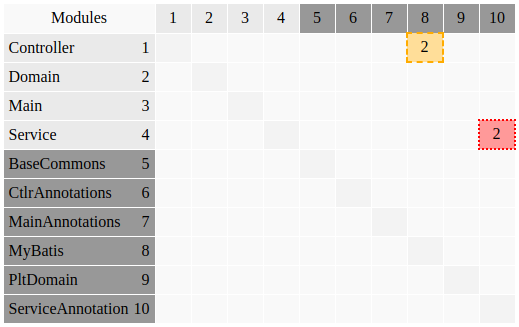
\includegraphics[width=0.65\textwidth]{figuras/violacoesAuthentication.png}
%\caption{Arquitetura de Microsserviços para o contexto de venda de produtos}
\caption{\textcolor{blue}{Authentication microservices's architectural project violations.}}
\label{fig:microservices}
\end{figure}
%--------------------------------------------
\newpage
\noindent\textbf{\textcolor{blue}{Authorization microservice}}
\label{sec:ApendiceAuthorization}
%--------------------------------------------
\begin{lstlisting}[style=colorido, caption={ \textcolor{blue}{Authorization microservice's architectural project specification.}},label={list:especArquiteturalAuthorization}
]
#Internal modules of the Authorization microservice
module Controller: br.com.microservices.authorization.controller.*
module Main: br.com.microservices.authorization.*
module ServiceInterface: br.com.microservices.authorization.services.[a-zA-Z]*Service
module ServiceImpl: br.com.microservices.authorization.services.[a-zA-Z]*Impl

#External modules
module Apache: org.apache.tomcat.**, org.apache.catalina.**, org.apache.logging.log4j.Logger
module BCMultitenancy: br.com.microservices. basecommons.multitenancy.**
module Beans: org.springframework.beans.**, org.springframework.context.**
module CtlrAnnotations: org.springframework.web.bind. annotation.RequestMapping, org.springframework.web.bind. annotation.RestController
module Jndi: org.springframework.jndi.**
module MainAnnotations: org.springframework.boot.context.properties.EnableConfigurationProperties, org.springframework.boot.autoconfigure.SpringBootApplication, org.springframework.cloud. client.discovery.EnableDiscoveryClient,  org.springframework.boot.SpringApplication
module ServiceAnnotation: org.springframework.stereotype.Service

#Structural Design Constraints SC's
#Only-can
only Controller, Service can-depend Service																																								"#SC1"
only Controller can-useannotation CtlrAnnotations																																		"#SC2"
only Service can-depend Jndi																																																							"#SC3"
only Main can-depend MainAnnotations																																															"#SC4"
	
#Can-only
Main can-depend-only $java, MainAnnotations, Apache																																"#SC5"@*@

#Cannot
Controller cannot-access Main																																																						"#SC6"
$system cannot-depend BCMultitenancy																																															"#SC7"
Service cannot-access Controller																																																			"#SC8"

#Must
ServiceImpl must-useannotation ServiceAnnotation																																			"#SC9"
ServiceImpl must-implement ServiceInterface																																								"#SC10"
Controller must-useannotation CtlrAnnotations																																						"#SC11"
\end{lstlisting}
%--------------------------------------------
%--------------------------------------------
\begin{figure}[ht]
\centering
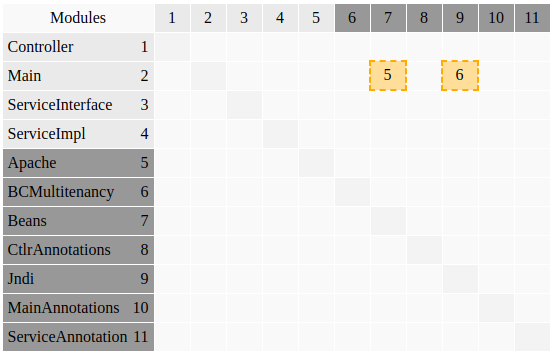
\includegraphics[width=0.75\textwidth]{figuras/violacoesAuthorization.png}
%\caption{Arquitetura de Microsserviços para o contexto de venda de produtos}
\caption{\textcolor{blue}{Authorization microservices's architectural project violations.}}
\label{fig:microservices}
\end{figure}
%--------------------------------------------

\newpage
\noindent\textbf{\textcolor{blue}{Conciliation Microservice}}
\label{sec:ApendiceConciliation}

%-------------------------------------------
\begin{lstlisting}[style=colorido, caption={\textcolor{blue}{Conciliation microservice's architectural project specification.}},label={list:especArquiteturalConciliation}
]
#Internal modules of the Conciliation microservice
module Controller: br.com.microservices.conciliation.controller.**
module DAO: br.com.microservices.conciliation.dao.**
module Domain: br.com.microservices.conciliation.domain.**
module ImplementDAO: br.com.microservices.conciliation.dao.[a-zA-Z]*DaoImpl
module Util: br.com.microservices.conciliation.util.**
module Main: br.com.microservices.conciliation.ConciliationApplication
module Service: br.com.microservices.conciliation.service.**
module Scheduled:  br.com.microservices.conciliation.scheduled.**

#External Modules
module AmazonSQS: com.amazonaws.services.sqs.AmazonSQS
module Beans: org.springframework.beans.**, org.springframework.stereotype.Component
module BCDAO: br.com.basecommons.daos.**
module BCDomain: br.com.basecommons.domain.*
module BCModel: br.com.basecommons.models.*
module BCMultitenancy: br.com.basecommons.multitenancy.**
module CtlrAnnotations: org.springframework.web.bind.annotation.RequestMapping, org.springframework.web.bind.annotation.RestController
module JPA: javax.persistence.**
module Logger: org.apache.logging.log4j.Logger
module MainAnnotations: org.springframework.boot.SpringApplication org.springframework.boot.context.properties.EnableConfigurationProperties, org.springframework.boot.autoconfigure.SpringBootApplication, org.springframework.cloud.client.discovery.EnableDiscoveryClient
module ServiceAnnotation: org.springframework.stereotype.Service
module SpringRepository: org.springframework.stereotype.Repository

#Structural Design Constraints SC's
#Only-can
only Controller can-useannotation CtlrAnnotations																																	"#SC1"
only Scheduled can-depend AmazonSQS																																															"#SC2"
only Service can-access DAO																																																							"#SC3"
only Controller, Service can-access Service																																							"#SC4"
only Main can-depend BCMultitenancy																																															"#SC5"
only DAO, Service can-depend BCDAO																																																"#SC6"
	
#Can-only
Util can-depend-only Util, $java, Logger																																										"#SC7"@*@
only Scheduled can-depend AmazonSQS																																															"#SC8"
Domain can-access-only BCModel, BCDomain, $java																																			"#SC9"
ImplementDAO can-depend-only JPA, Hibernate, $java, SpringRepository, BCModel					"#SC10"
Main can-access-only Controller, MainAnnotations, Logger,  $java																			"#SC11"

#Cannot
Domain cannot-depend JPA																																																										"#SC12"
Controller cannot-access DAO																																																						"#SC13"

#Must
Main must-useannotation MainAnnotations																																											"#SC14"
ImplementDAO must-depend SpringRepository																																									"#SC15"
Service must-useannotation ServiceAnnotation																																						"#SC16"


	
\end{lstlisting}
%--------------------------------------------
%--------------------------------------------
\begin{figure}[ht]
\centering
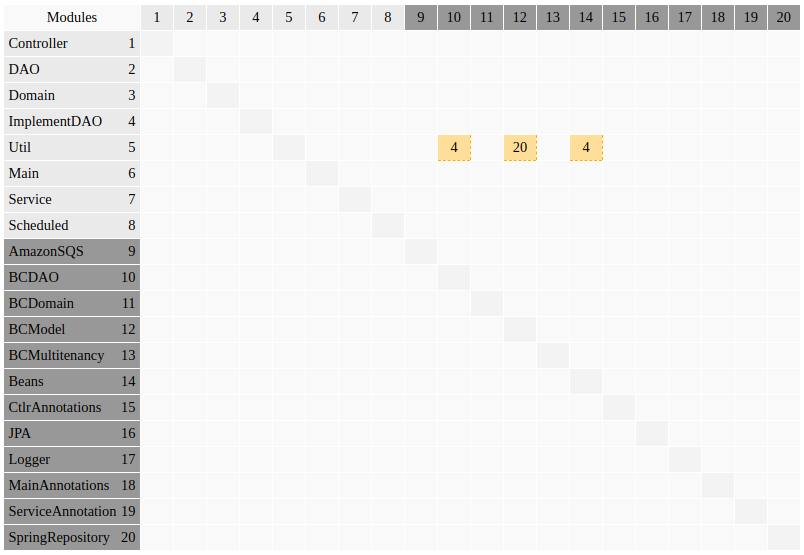
\includegraphics[width=0.75\textwidth]{figuras/violacoesConciliation.png}
%\caption{Arquitetura de Microsserviços para o contexto de venda de produtos}
\caption{\textcolor{blue}{Conciliation microservices's architectural project violations.}}
\label{fig:microservices}
\end{figure}
%--------------------------------------------

\newpage
\noindent\textbf{\large{\textcolor{blue}{Dashboard}}}
\label{sec:ApendiceDashboard}


%--------------------------------------------
\vspace{0.2cm}
\begin{lstlisting}[style=colorido, caption={\textcolor{blue}{Dashboard microservice's architectural project specification.}},label={list:especArquiteturalDashboard}
]
module Controller: br.com.microservices.dashboard.controller.*
module DAO: br.com.microservices.dashboard.dao.**
module DAOInterface: br.com.microservices.dashboard.dao.[a-zA-Z]*Dao
module Service: br.com.microservices.dashboard.service.*

#External Modules
module BCController: br.com.basecommons.controller.**
module BCModel: br.com.basecommons.models.**
module CtlrAnnotations: org.springframework.web.bind.annotation.RequestMapping, org.springframework.web.bind. annotation.RestController
module Hibernate: org.hibernate.**
module MainAnnotations: org.springframework.boot.context.properties.EnableConfigurationProperties, org.springframework.boot.autoconfigure.SpringBootApplication, org.springframework.cloud.client.discovery.EnableDiscoveryClient, org.springframework.boot.SpringApplication
module ServiceAnnotation: org.springframework.stereotype.Service
module SpringRepository: org.springframework.stereotype.Repository

#Structural Design Constraints SC's
#Only-can
only Controller can-useannotation CtlrAnnotations																																		"#SC1"
only Controller can-depend BCController																																												"#SC2"
only Main can-depend BCMultitenancy																																																"#SC3"
only Service, DAO can-access DAO																																																			"#SC4"

#Can-only
ImplementDAO can-depend-only JPA, Hibernate, $java, SpringRepository, BCModel						"#SC5"

#Cannot
Controller cannot-access DAO																																																							"#SC6"
Service cannot-depend Controller																																																			"#SC7"

#Must
Main must-useannotation MainAnnotations																																												"#SC8"
Controller must-access Service																																																					"#SC9"@*@
ImplementDAO must-implement DAOInterface																																											"#SC10"
ImplementDAO must-depend SpringRepository																																										"#SC11"
Service must-useannotation ServiceAnnotation																																							"#SC12"


\end{lstlisting}
%--------------------------------------------
%--------------------------------------------
\begin{figure}[ht]
\centering
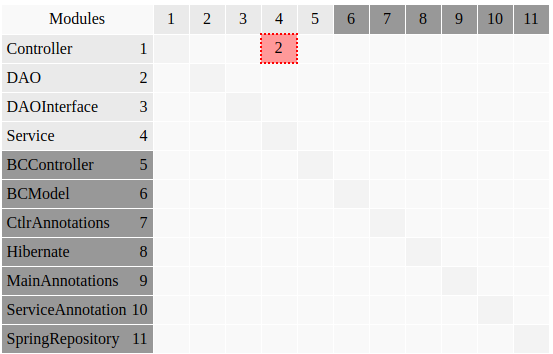
\includegraphics[width=0.7\textwidth]{figuras/violacoesDashboard.png}
%\caption{Arquitetura de Microsserviços para o contexto de venda de produtos}
\caption{\textcolor{blue}{Dashboard microservices's architectural project violations.}}
\label{fig:microservices}
\end{figure}
%--------------------------------------------

\newpage
\noindent\textbf{\large{\textcolor{blue}{Entries microservice}}}
\label{sec:ApendiceEntries}


%--------------------------------------------
\begin{lstlisting}[style=colorido, caption={ \textcolor{blue}{Entries microservice's architectural project specification.}},label={list:especArquiteturalEntries}
]
 #Internal modules of the Entries microservice
module Util: br.com.microservices.entries.utils.*
module Controller:  br.com.microservices.entries.controller.*
module DAO: br.com.microservices.entries.dao.*
module ImplementDAO: br.com.microservices.entries.dao. [a-zA-Z]*DaoImpl
module Main: br.com.microservices.entries.EntriesApplication
module Model: br.com.microservices.entries.model.**, br.com.microservices.entries.model.**, br.com.microservices.entries.models.**
module Service: br.com.microservices.entries.service.**
module ServiceImplement: br.com.microservices.entries.service.*[a-zA-Z]*ServiceImpl
module Serializer: br.com.microservices.entries.serializer.*

#External Modules
module BCMultitenancy: br.com.basecommons.multitenancy.**	
module CtlrAnnotations: org.springframework.web.bind. annotation.RequestMapping, org.springframework.web.bind. annotation.RestController
module Hibernate: org.hibernate.**
module JPA: javax.persistence.**
module MainAnnotations: org.springframework.boot.SpringApplication org.springframework.boot.context.properties.EnableConfigurationProperties, org.springframework.boot.autoconfigure.SpringBootApplication, org.springframework.cloud.client.discovery.EnableDiscoveryClient
module Serializable: java.io.Serializable
module ServiceAnnotation: org.springframework.stereotype.Service	
module SpringRepository: org.springframework.stereotype.Repository

#Structural Design Constraints SC's
#Only-can 
only Controller can-useannotation CtlrAnnotations																																	"#SC1"
only Controller, Service can-access Service																																							"#SC2"
only Service can-access DAO																																																							"#SC3"
only Main can-depend BCMultitenancy																																															"#SC4"@*@

#Can-only
Util can-depend-only Util, $java																																																		"#SC5"@*@
ImplementDAO can-depend-only JPA, Hibernate, SpringRepository, $java														"#SC6"

#Cannot
Controller cannot-access DAO, BCDAO																																															"#SC7"@*@

#Must
Main must-useannotation MainAnnotations																																											"#SC8"
Controller must-useannotation CtlrAnnotations																																					"#SC9"
Service must-useannotation ServiceAnnotation																																						"#SC10"
Model, Serializer must-implement Serializable																																					"#SC11"@*@
ImplementDAO must-implement SpringRepository																																						"#SC12"

\end{lstlisting}
%--------------------------------------------
%--------------------------------------------
\begin{figure}[ht]
\centering
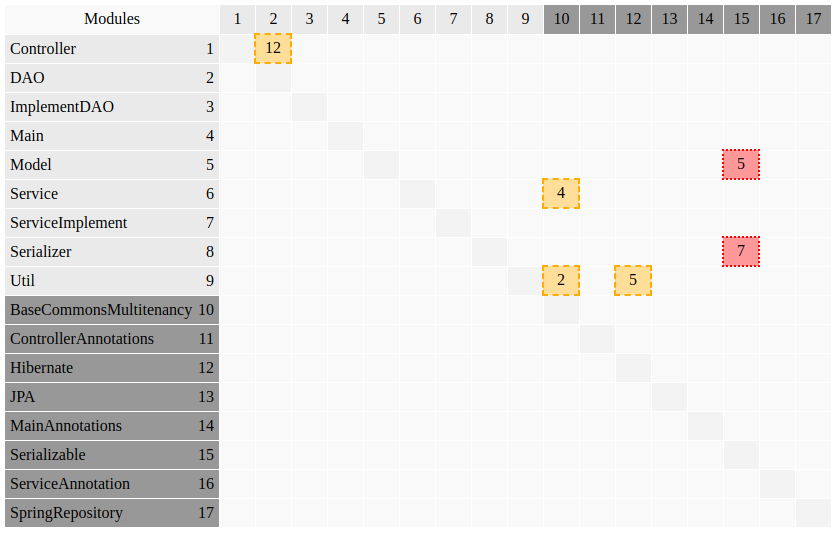
\includegraphics[width=0.7\textwidth]{figuras/violacoesEntries.png}
%\caption{Arquitetura de Microsserviços para o contexto de venda de produtos}
\caption{\textcolor{blue}{Entries microservices's architectural project violations.}}
\label{fig:microservices}
\end{figure}
%--------------------------------------------


\newpage
\noindent\textbf{\large{\textcolor{blue}{FileLoad microservice}}}
\label{sec:ApendiceFileLoad}


%--------------------------------------------
\begin{lstlisting}[style=colorido, caption={\textcolor{blue}{FileLoad microservice's architectural project specification.}},label={list:especArquiteturalFileLoad}
]
#Internal modules of the  FileLoad microservice
module DAO: br.com.microservices.fileload.daos.*
module DAOInterface: br.com.microservices.fileload.daos.[a-zA-Z]*Dao
module ImplementDAO: br.com.microservices.fileload.daos.[a-zA-Z]*DaoImpl
module Main: br.com.microservices.fileload.*
module Model: br.com.microservices.fileload.models.**
module Service: br.com.microservices.fileload.services.*

#External Modules
module BCDAO: br.com.basecommons.daos.**
module BCModel: br.com.basecommons.basecommons.models.*
module BCMultitenancy: br.com.basecommons.multitenancy.**
module Beans: javax.validation.**
module DataSource: org.springframework.boot.autoconfigure.
jdbc.DataSourceAutoConfiguration
module Hibernate: org.hibernate.**
module JPA: javax.persistence.**
module MainAnnotations: org.springframework.boot.SpringApplication, 
org.springframework.boot.context.properties.EnableConfigurationProperties, org.springframework.boot.autoconfigure.SpringBootApplication, org.springframework.cloud.client.discovery.EnableDiscoveryClient
module Serializable: java.io.Serializable
module ServiceAnnotation: org.springframework.stereotype.Service
module SpringRepository: org.springframework.stereotype.Repository

#Structural Design Constraints SC's
#Only-can 
only Model, DAO can-depend JPA, Beans																																													"#SC1"
only Main can-useannotation MainAnnotations, DataSource																											"#SC2"
only Main can-depend BCMultitenancy																																															"#SC3"
only Service can-useannotation ServiceAnnotation																																		"#SC4"

#Can-only
ImplementDAO can-depend-only JPA, Hibernate, $java, SpringRepository, BCModel					"#SC5"
	
#Cannot
Main cannot-depend DAO, Model, BCDAO, JPA 																																								"#SC6"@*@
Service cannot-access Main																																																								"#SC7"

#Must
ImplementDAO must-implement DAOInterface																																										"#SC8"
ImplementDAO must-depend SpringRepository																																									"#SC9"
Model must-implement Serializable																																																	"#SC10"@*@
Service must-useannotation ServiceAnnotation																																						"#SC11"
\end{lstlisting}
%--------------------------------------------
%--------------------------------------------
\begin{figure}[ht]
\centering
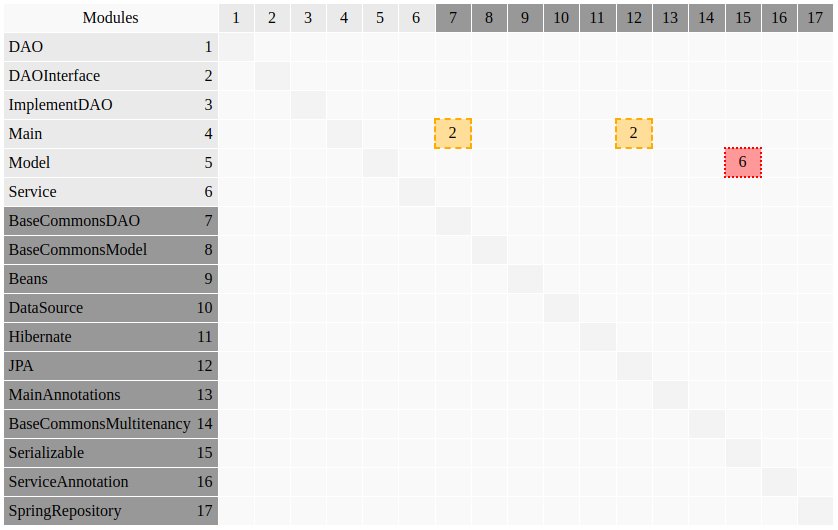
\includegraphics[width=0.7\textwidth]{figuras/violacoesFileLoad.png}
\vspace{-0.2cm}
\caption{\textcolor{blue}{FileLoad microservices's architectural project violations.}}
\label{fig:microservices}
\end{figure}
%--------------------------------------------

% \newpage
\noindent\textbf{\large{\textcolor{blue}{FileProcess microservice}}}
\label{sec:ApendiceFileProccess}


%--------------------------------------------
\begin{lstlisting}[style=colorido, caption={\textcolor{blue}{FileProcess microservice's architectural project specification.}},label={list:especArquiteturalFileProccess}
]
#Internal modules of the FileProcess microservice
module DAO: br.com.microservices.process.dao.**
module DAOInterface: br.com.microservices. process.dao.[a-zA-Z]*Dao
module ImplementDAO: br.com.microservices. process.dao.[a-zA-Z]*DaoImpl
module Main: br.com.microservices.process.Application
module Model: br.com.microservices.model.**
module Scheduling: br.com.microservices.schedule.**
module Service: br.com.microservices.service.**
module Util: br.com.microservices.process.util.**

#External Modules
module AmazonService: com.amazonaws.services.**
module BCDomain: equals.gestaofinanceira.microservices.cba. basecommons.domain.**
module BCUtil: br.com.basecommons.utils.**
module BCMultitenancy: br.com.basecommons.multitenancy.**
module JPA: javax.persistence.**
module Logger: org.apache.logging.log4j.Logger
module MainAnnotations: org.springframework.boot.SpringApplication, org.springframework.boot.context.properties.EnableConfigurationProperties, org.springframework.boot.autoconfigure.SpringBootApplication, org.springframework.cloud.client.discovery.EnableDiscoveryClient
module ScdAnnotation: org.springframework.scheduling. annotation.EnableScheduling
module ScdFramework: org.springframework.scheduling.**
module Serializable: java.io.Serializable
module ServiceAnnotation: org.springframework.stereotype.Service
module SpringBeans: org.springframework.beans.**
module SpringRepository: org.springframework.stereotype.Repository

#Structural Design Constraints SC's
#Only-can
only Main can-useannotation MainAnnotations																																						"#SC1"
only Scheduling can-access ScdFramework																																										"#SC2"
only Main can-depend BCMultitenancy																																														"#SC3"
only DAO, Model can-depend JPA																																				"#SC4"@*@
only Service, Scheduling can-depend AmazonService																																"#SC5"

#Restricoes  can-only
Util can-depend-only Util, BCUtil, $java, Logger																																	"#SC6"@*@
    
#Cannot
Service cannot-depend Controller																																																	"#SC7"
    
#Must
Main must-useannotation MainAnnotations																																										"#SC8"
Service must-useannotation ServiceAnnotation																																					"#SC9"
ImplementDAO must-implement DAOInterface, SpringRepository																							"#SC10"
Model must-implement Serializable																																																"#SC11"@*@
Scheduling must-depend ScdFramework																																														"#SC12"
Scheduling must-useannotation ScdAnnotation																																						"#SC13"

\end{lstlisting}

%--------------------------------------------
%--------------------------------------------
\begin{figure}[ht]
\centering
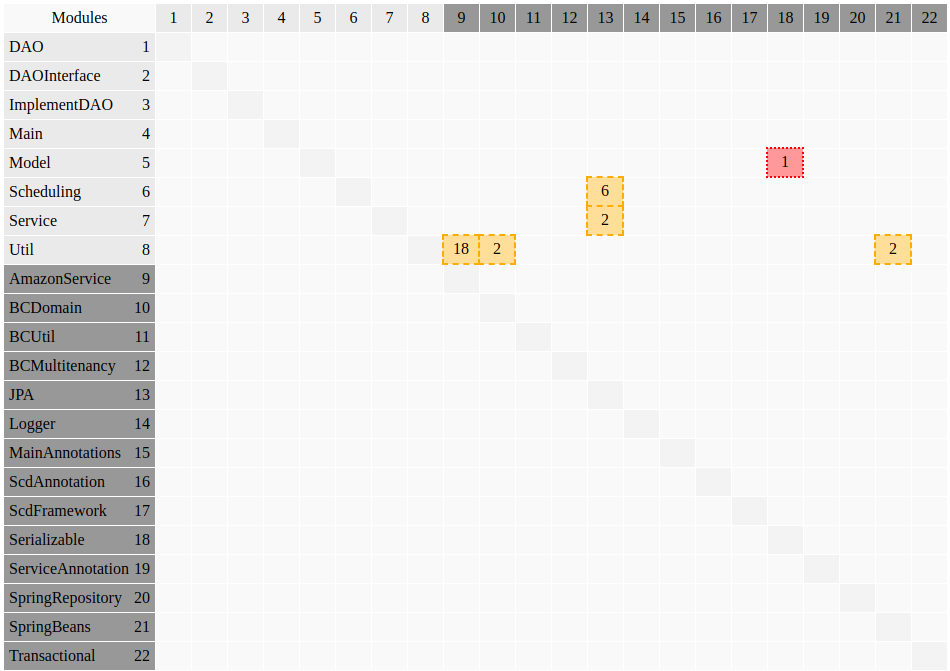
\includegraphics[width=0.75\textwidth]{figuras/violacoesFileProccess.png}
\caption{\textcolor{blue}{FileProcess microservices's architectural project violations.}}
\label{fig:microservices}
\end{figure}
%--------------------------------------------


% \newpage
\noindent\textbf{\large{\textcolor{blue}{Reports microservice}}}
\label{sec:ApendiceReports}

%--------------------------------------------
\begin{lstlisting}[style=colorido,caption={\textcolor{blue}{Reports microservice's architectural project specification.}},label={list:especArquiteturalReports}
]
#Internal modules of the Reports microservice
module Controller: br.com.microservices.reports.controller.**
module Main: br.com.microservices.reports.ReportsApplication
module Serializer: br.com.microservices.reports.serializer.**
module Service: br.com.microservices.reports.service.**

#External Modules
module BCController: br.com.basecommons.controller.BaseController
module BCMultitenancy: br.com.basecommons.basecommons.multitenancy.properties.MultitenancyProperties
module CtlrAnnotations: org.springframework.web.bind.annotation.RequestMapping, org.springframework.web.bind.annotation.RestController, ControllerAnnotations.**
module JSONSerializer: flexjson.JSONSerializer.*
module MainAnnotations: org.springframework.boot.SpringApplication,  org.springframework.boot.context.properties.EnableConfigurationProperties, org.springframework.boot.autoconfigure.SpringBootApplication, org.springframework.cloud.client.discovery.EnableDiscoveryClient
module ServiceAnnotation: org.springframework.stereotype.Service

#Structural Design Constraints SC's
#Only-can
only Controller can-useannotation CtlrAnnotations																																	"#SC1"
only Main can-depend BCMultitenancy																																															"#SC2"
only Main can-useannotation MainAnnotations																																							"#SC3"

#Cannot
Service cannot-access Controller																																																		"#SC4"

#Must	
Main must-useannotation MainAnnotations																																											"#SC5"
Controller must-useannotation CtlrAnnotations																																					"#SC6"@*@
Controller must-extend BCController																																															"#SC7"@*@
Service must-useannotation ServiceAnnotation																																						"#SC8"
Serializer must-depend JSONSerializer																																													"#SC9"@*@

\end{lstlisting}
%--------------------------------------------
%--------------------------------------------
\begin{figure}[ht]
\centering
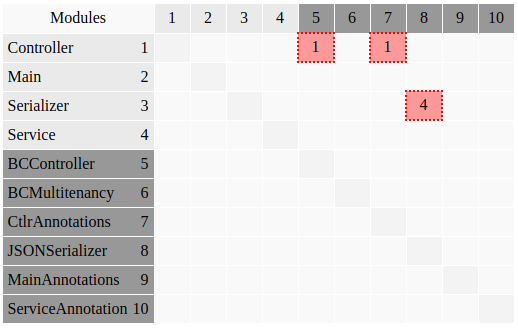
\includegraphics[width=0.65\textwidth]{figuras/violacoesReports.png}
\caption{\textcolor{blue}{Reports microservices's architectural project violations.}}
\label{fig:microservices}
\end{figure}
%--------------------------------------------

\newpage
\noindent\textbf{\large{\textcolor{blue}{Summary microservice}}}
\label{sec:ApendiceSummary}

%--------------------------------------------
\begin{lstlisting}[style=colorido, caption={\textcolor{blue}{Summary microservice's architectural project specification.}},label={list:especArquiteturalSummary}
]
#Internal modules of the Summary microservice
module BaseService:  br.com.microservices.summary.service.BaseService
module Controller:  br.com.microservices.summary.controller.*
module DAO: br.com.microservices.summary.dao.*
module DAOInterface: br.com.microservices.summary.dao.[a-zA-Z]*Dao
module ImplementDAO: br.com.microservices.summary.dao.[a-zA-Z]*Impl
module Main: br.com.microservices.summary.SummaryApplication
module Service: br.com.microservices.summary.service.*
module ServiceSubClass: br.com.microservices.summary.service.AtributoService, br.com.microservices.summary.service.ConciliacaoService, br.com.microservices.summary.service.TreegridService
module Stream: br.com.microservices.summary.stream.*
module Util: br.com.microservices.summary.util.**

#External Modules
module BCMultitenancy: br.com.basecommons.multitenacy.**
module CtlrAnnotations: org.springframework.web.bind.annotation.RequestMapping, org.springframework.web.bind. annotation.RestController
module MainAnnotations:  org.springframework.boot.SpringApplication, org.springframework.boot.context.properties.EnableConfigurationProperties, org.springframework.boot.autoconfigure.SpringBootApplication, org.springframework.cloud.client.discovery.EnableDiscoveryClient
module Repository: org.springframework.stereotype.Repository
module ServiceAnnotation: org.springframework.stereotype.Service

#Structural Design Constraints SC's
#Only-can
only Service can-useannotation ServiceAnnotation																																		"#SC1" 
only Controller can-useannotation CtlrAnnotations																																	"#SC2"
only Main can-useannotation MainAnnotations																																							"#SC3"
only Main can-depend BCMultitenancy																																															"#SC4"

#Can-only	
Util can-access-only Util, $java																																																		"#SC5"

#Must
Main must-useannotation MainAnnotations																																											"#SC6"
Service must-useannotation ServiceAnnotation																																						"#SC7"@*@
Controller must-useannotation CtlrAnnotations																																					"#SC8"@*@
ServiceSubClass must-extend BaseService																																											"#SC9"
ImplementDAO must-implement DAOInterface																																										"#SC10"
ImplementDAO must-useannotation Repository																																								"#SC11"
Controller must-access Stream																																																					"#SC12"
\end{lstlisting}
%--------------------------------------------
%--------------------------------------------
\begin{figure}[ht]
\centering
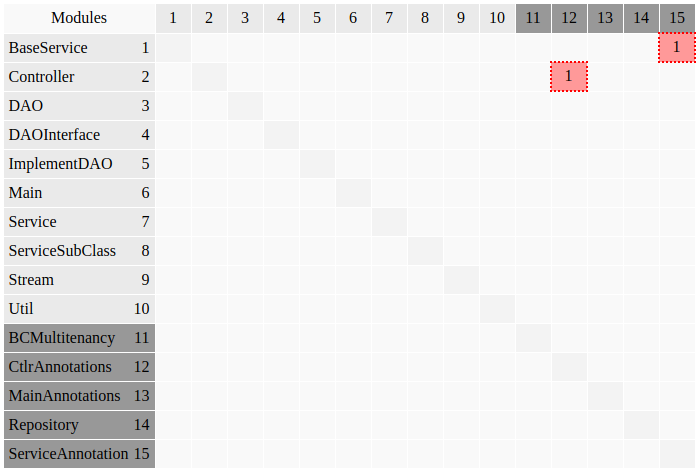
\includegraphics[width=0.7\textwidth]{figuras/violacoesSummary.png}
\caption{\textcolor{blue}{Summary microservices's archictetural project violations.}}
\label{fig:microservices}
\end{figure}
%--------------------------------------------
% 
%--------------------------------------------
% \newpage
% % Please add the following required packages to your document preamble:
% % \usepackage{multirow}
% \begin{table}[]
%   \begin{adjustbox}{width=\textwidth}

% \footnotesize
% \begin{tabular}{|l|l|l|l|l|}
% \hline
% Módulo                                                                           & Restrição                                                                                                                                                                                                         & Viol.              & Comunicação violada                                                                                                                         & Local da violação                                                                                         \\ \hline
% \multirow{3}{*}{Assigment}                                                       & \multirow{2}{*}{Assigment can-communicate-only reports}                                                                                                                                                           & \multirow{2}{*}{2} & \begin{tabular}[c]{@{}l@{}}Assigment communicates entries \\ using /cliente/\$clientId/tarefas\end{tabular}                                 & \begin{tabular}[c]{@{}l@{}}\$system/assignment/assignment.js\\ (linha …)\end{tabular}                     \\ \cline{4-5} 
%                                                                                  &                                                                                                                                                                                                                   &                    & \begin{tabular}[c]{@{}l@{}}Assigment communicate entries \\ using cliente/\$clientId/\\ tarefaTipoVinculo/\$tarefaId\end{tabular}             & \begin{tabular}[c]{@{}l@{}}\$system/assignment/assignment.js \\ (linha ..)\end{tabular}                   \\ \cline{2-5} 
%                                                                                  & Assigment must-communicate reports                                                                                                                                                                                &                    & --                                                                                                                                          & --                                                                                                        \\ \hline
% \multirow{2}{*}{\begin{tabular}[c]{@{}l@{}}Occurrence-\\ Report\end{tabular}}    & \begin{tabular}[c]{@{}l@{}}OccurrenceReport can-communicate-only \\ reports\end{tabular}                                                                                                                          & \multirow{2}{*}{1} & \begin{tabular}[c]{@{}l@{}}OccurrenceReport communicates \\ entries using /cliente/\$clientId/\\ atributos\end{tabular}                     & \begin{tabular}[c]{@{}l@{}}\$system/occurrenceReport/\\ occurrenceReport.js (linha ..)\end{tabular}       \\ \cline{2-2} \cline{4-5} 
%                                                                                  & \begin{tabular}[c]{@{}l@{}}OccurrenceReport must-communicate \\ reports\end{tabular}                                                                                                                              &                    & --                                                                                                                                          & --                                                                                                        \\ \hline
                                                                                 
% \multirow{2}{*}{\begin{tabular}[c]{@{}l@{}}Financial-\\ Movements\end{tabular}}    & \begin{tabular}[c]{@{}l@{}}FinancialMovements can-communicate-only \\ reports\end{tabular}                                                                                                                          & \multirow{2}{*}{1} & \begin{tabular}[c]{@{}l@{}}FinancialMovements communicate \\entries using /cliente/\$clientId/atributos
% \end{tabular}                     & \begin{tabular}[c]{@{}l@{}}\$system/financialMovements/\\financialMovements.js (linha …)\end{tabular}       \\ \cline{2-2} \cline{4-5} 
%                                                                                  & \begin{tabular}[c]{@{}l@{}}
% FinancialMovements must-communicate \\reports 
% \end{tabular}                                                                                                                              &                    & --                                                                                                                                          & --                                                                                                        \\ \hline
% \multirow{5}{*}{\begin{tabular}[c]{@{}l@{}}Conciliation-\\ Report\end{tabular}}  & \multirow{4}{*}{\begin{tabular}[c]{@{}l@{}}ConciliationReport can-communicate-only\\ reports\end{tabular}}                                                                                                        & \multirow{4}{*}{4} & \begin{tabular}[c]{@{}l@{}}ConciliationReport communicates \\ summary using /cliente/\$clientId/\\ detalheConciliacaoDownload\end{tabular}  & \begin{tabular}[c]{@{}l@{}}\$system//conciliationReport/\\ conciliationReport.js (linha ..)\end{tabular}  \\ \cline{4-5} 
%                                                                                  &                                                                                                                                                                                                                   &                    & \begin{tabular}[c]{@{}l@{}}ConciliationReport communicates\\  summary using /cliente/\$clientId/\\ detalheConciliacao\end{tabular}          & \begin{tabular}[c]{@{}l@{}}\$system//conciliationReport/\\ conciliationReport.js (linha ..)\end{tabular}  \\ \cline{4-5} 
%                                                                                  &                                                                                                                                                                                                                   &                    & \begin{tabular}[c]{@{}l@{}}ConciliationReport communicates \\ entries using /cliente/\$clientId/\\ categorias\end{tabular}                  & \begin{tabular}[c]{@{}l@{}}\$system//conciliationReport/\\ conciliationReport.js\end{tabular}             \\ \cline{4-5} 
%                                                                                  &                                                                                                                                                                                                                   &                    & \begin{tabular}[c]{@{}l@{}}ConciliationReport communicates\\ entries using  /cliente/\$clientId/\\ atributos\end{tabular}                   & \begin{tabular}[c]{@{}l@{}}\$system//conciliationReport/\\ conciliationReport.js (linha …)\end{tabular}   \\ \cline{2-5} 
%                                                                                  & \begin{tabular}[c]{@{}l@{}}ConciliationReport must-communicate \\ reports\end{tabular}                                                                                                                            & --                 & --                                                                                                                                          & --                                                                                                        \\ \hline
% \multirow{3}{*}{AuditLog}                                                        & only AuditLog can-communicate audit                                                                                                                                                                               & --                 & --                                                                                                                                          &                                                                                                           \\ \cline{2-5} 
%                                                                                  & AuditLog can-communicate-only audit                                                                                                                                                                               & 1                  & \begin{tabular}[c]{@{}l@{}}AuditLog communicates entries\\  using /entidades\end{tabular}                                                   & \begin{tabular}[c]{@{}l@{}}\$system/auditLog/audits/\\ audits.js (linha …)\end{tabular}                   \\ \cline{2-5} 
%                                                                                  & AuditLog must-communicate audit                                                                                                                                                                                   &                    & --                                                                                                                                          & --                                                                                                        \\ \hline
% \multirow{5}{*}{\begin{tabular}[c]{@{}l@{}}Conciliation-\\ Summary\end{tabular}} & \multirow{2}{*}{\begin{tabular}[c]{@{}l@{}}only ConciliationSummary can-communicate\\ summary\end{tabular}}                                                                                                       & \multirow{2}{*}{2} & \begin{tabular}[c]{@{}l@{}}ConciliationReport communicates\\ summary using /cliente/\$clientId/\\ detalheConciliacao\end{tabular}           & \begin{tabular}[c]{@{}l@{}}\$system/conciliationReport/\\ conciliationReport.js (linha ..)\end{tabular}   \\ \cline{4-5} 
%                                                                                  &                                                                                                                                                                                                                   &                    & \begin{tabular}[c]{@{}l@{}}ConciliationReport communicates\\ summary using /cliente/\$clientId/\\ detalheConciliacaoDownload\end{tabular}   & \begin{tabular}[c]{@{}l@{}}\$system/conciliationReport/\\ conciliationReport.js (linha ..)\end{tabular}   \\ \cline{2-5} 
%                                                                                  & \multirow{2}{*}{\begin{tabular}[c]{@{}l@{}}ConciliationSummary can-communicate-only\\ summary\end{tabular}}                                                                                                       & \multirow{2}{*}{2} & \begin{tabular}[c]{@{}l@{}}ConciliationSummary communicates\\ reports using /cliente/\$clientId/\\ resumoConciliacao\end{tabular}           & \begin{tabular}[c]{@{}l@{}}\$system/conciliationSummary/\\ conciliationSummary.js (linha ..)\end{tabular} \\ \cline{4-5} 
%                                                                                  &                                                                                                                                                                                                                   &                    & \begin{tabular}[c]{@{}l@{}}ConciliationSummary communicates\\ entries  using /cliente/\$clientId/atributos\end{tabular}                     & \begin{tabular}[c]{@{}l@{}}\$system/conciliationSummary.js \\ (linha …)\end{tabular}                      \\ \cline{2-5} 
%                                                                                  & \begin{tabular}[c]{@{}l@{}}ConciliationSummary must-communicate\\ summary\end{tabular}                                                                                                                            & 1                  & --                                                                                                                                          & --                                                                                                        \\ \hline
% \multirow{4}{*}{\begin{tabular}[c]{@{}l@{}}Manual-\\ Conciliation\end{tabular}}  & \begin{tabular}[c]{@{}l@{}}only ManualConciliation can-communicate \\ conciliation\end{tabular}                                                                                                                   & --                 & --                                                                                                                                          & --                                                                                                        \\ \cline{2-5} 
%                                                                                  & \multirow{2}{*}{\begin{tabular}[c]{@{}l@{}}ManualConciliation can-communicate-only \\ conciliation\end{tabular}}                                                                                                  & \multirow{2}{*}{2} & \begin{tabular}[c]{@{}l@{}}ManualConciliation communicate \\ entries using /cliente/\$clientId/atributos\end{tabular}                       & \begin{tabular}[c]{@{}l@{}}\$system/manualConciliation/\\ allotmentData.js (linha..)\end{tabular}         \\ \cline{4-5} 
%                                                                                  &                                                                                                                                                                                                                   &                    & \begin{tabular}[c]{@{}l@{}}ManualConciliation communicate \\ entries using  /cliente/\$clientId/\\ categorias\end{tabular}                  & \begin{tabular}[c]{@{}l@{}}\$system/manualConciliation/\\ allotmentData.js (linha ..)\end{tabular}        \\ \cline{2-5} 
%                                                                                  & \begin{tabular}[c]{@{}l@{}}ManualConciliation must-communicate \\ conciliation\end{tabular}                                                                                                                       & --                 & --                                                                                                                                          & --                                                                                                        \\ \hline
% \multirow{2}{*}{\begin{tabular}[c]{@{}l@{}}Processed-\\ Files\end{tabular}}      & \multirow{2}{*}{\begin{tabular}[c]{@{}l@{}}ProcessedFiles cannot-communicate \\ authorization, authentication, audit,\\ conciliation, entries, reports, dashboard,\\ summary, fileProcces, fileLoad\end{tabular}} & \multirow{2}{*}{2} & \begin{tabular}[c]{@{}l@{}}ProcessedFiles communicate reports \\ using /cliente/\$clientId/\\ arquivoProcessado/\$idProcessament\end{tabular} & \begin{tabular}[c]{@{}l@{}}\$system/processedFiles/\\ processedFiles.js (linha .)\end{tabular}            \\ \cline{4-5} 
%                                                                                  &                                                                                                                                                                                                                   &                    & \begin{tabular}[c]{@{}l@{}}ProcessedFiles communicate reports \\ using /cliente/\$clientId/\\ arquivosProcessados\end{tabular}              & \begin{tabular}[c]{@{}l@{}}\$system//processedFiles/\\ processedFiles.js (linha ..)\end{tabular}          \\ \hline
% \end{tabular}
%   \end{adjustbox}

% \end{table}
%--------------------------------------------------------------
%--------------------------------------------
\end{document}
